\documentclass[12pt, twoside]{article}
\usepackage[francais]{babel}
\usepackage[T1]{fontenc}
\usepackage[latin1]{inputenc}
\usepackage[left=7mm, right=1cm, top=1cm, bottom=7mm]{geometry}
\usepackage{float}
\usepackage{graphicx}
\usepackage{array}
\usepackage{multirow}
\usepackage{amsmath,amssymb,mathrsfs}
\usepackage{soul}
\usepackage{textcomp}
\usepackage{eurosym}
 \usepackage{variations}
\usepackage{tabvar}

\begin{document}


\section*{\center{Aide individualis�e: Domaine de d�finition}}

\subsection*{Intervalles}

\begin{enumerate}
  \item On note $D_{1}$ l'ensemble des r�els diff�rents de 4. Repr�senter
  l'ensemble $D_{1}$ sur la droite gradu�e.
  
  \bigskip
  
  \bigskip
  
 On a: $D_{1}=]- \infty$; \ldots \ldots $\cup$ \ldots \ldots ;$+\infty[$ 
 
 On peut �crire aussi:  $D_{1}= \mathbb{R}$ \textbackslash  \ldots \ldots
 \item On note $D_{2}$ l'ensemble des r�els diff�rents de -1 et de 6.
 Repr�senter l'ensemble $D_{2}$ sur la droite gradu�e.
  
  \bigskip
  
  \bigskip
  
 On a: $D_{2}=$ \ldots \ldots \ldots \ldots \ldots \ldots \ldots \ldots \ldots
 \ldots\ldots (avec des intervalles)
 
\qquad \qquad \quad $=$ \ldots \ldots \ldots \ldots \ldots (avec le symbole $\mathbb{R}$)
 
 
 \item On note $D_{3}$ l'ensemble des r�els strictement positifs.
 Repr�senter l'ensemble $D_{3}$ sur la droite gradu�e.
  
  \bigskip
  
  \bigskip
  
 On a: $D_{3}=$ \ldots \ldots \ldots \ldots  (avec des intervalles)
 
\qquad \qquad \quad $=$ \ldots \ldots \ldots \ldots \ldots (avec le symbole
$\mathbb{R}$)
 
 \end{enumerate}

\subsection*{Domaine de d�finition}

\ul{M�thode}:

\enskip

\fbox{ \begin{minipage}{18cm}
 D�terminer l'ensemble de d�finition d'une fonction $f$ c'est
trouver l'ensemble des $x$ pour lesquels on peut calculer $f(x)$ (c'est-�-dire
les $x$ tels que $f(x)$ a du sens).
\end{minipage}
}

\enskip

On sait que: diviser par  \ldots \ldots n'est pas possible et la racine d'un
nombre \ldots \ldots \ldots n'existe pas.

\enskip

\fbox{
\begin{minipage}{12cm}

\begin{itemize}
 \item [$\bullet$] Le calcul de $\dfrac{A(x)}{B(x)}$ n'est possible que si $B(x)
\ldots \ldots \ldots$.

\enskip

\item  [$\bullet$] Le calcul de $\sqrt{A(x)}$ n'est possible que si $A(x)
\ldots \ldots \ldots$.
\end{itemize}
\end{minipage}
}


\bigskip

\ul{Exemples}: D�terminons l'ensemble de d�finitions de chaque fonction.
\begin{enumerate}
  \item $f(x)=\dfrac{1}{x-5}$. 
  
  \enskip
  
  On ne peut pas avoir \ldots \ldots \ldots $=0$.
  
  Recherche de la valeur interdite: \ldots \ldots \ldots
  
  On peut calculer $f(x)$ pour tous les r�els $x$ sauf pour $x=\ldots$.
   
  \enskip
  
    
   Donc $\mathcal{D}_{f}=$ \ldots \ldots \ldots \ldots \ldots (avec des
   intervalles)
  
  \qquad \qquad  $=$ \ldots \ldots \ldots (avec le symbole
$\mathbb{R}$)
\item $g(x)= \sqrt{x-7}$

\enskip
  
  On ne peut pas avoir \ldots \ldots \ldots $<0$.
  
  IL faut donc chercher les $x$ tels que  \ldots \ldots \ldots \ldots$>0$
  c'est-�-dire $x$ \ldots \ldots
  
  On peut calculer $g(x)$ seulement pour $x$ \ldots \ldots \ldots
   
  \enskip
  
    
   Donc $\mathcal{D}_{f}=$ \ldots \ldots \ldots \ldots \ldots (avec des
   intervalles)
  
  \qquad \qquad  $=$ \ldots \ldots \ldots (avec le symbole
$\mathbb{R}$)

\item  $h(x)=\sqrt{(x-3)(6-x)}$

L'ensemble de d�finition de $h$ est l'ensemble des
r�els $x$ tels que \ldots \ldots \ldots \ldots \ldots \ldots \ldots \ldots.

 On doit donc r�soudre \ldots\ldots \ldots \ldots \ldots \ldots \ldots \ldots.

 C'est une in�quation-\ldots \ldots \ldots \ldots; il faut donc faire un \ldots
 \ldots \ldots \ldots \ldots \ldots \ldots \ldots.
 
 \medskip
 
 \textbf{METHODE:}

\begin{enumerate}
  \item On cherche les valeurs qui annulent chaque facteur:
  
 $x+3=0$ \qquad \qquad \qquad \qquad \qquad $6-x=0$ \\
 $\Leftrightarrow$ $x=\ldots$ \qquad \qquad \qquad \qquad \qquad $\Leftrightarrow$
 $x=\ldots$
 
  \item On place les valeurs dans l'ordre croissant sur la ligne des $x$. On
  met les ``$0$'' � l'endroit correspondant:
  
  Dans notre cas: lorsque $x=-3$, $x+3=0$. On place donc le z�ro dans la
  colonne -3 et sur la ligne $x+3$.
  
  
  On fait de m�me pour 6: lorsque $x=6$, $6-x=0$. on place donc le z�ro dans la
  colonne 6 et sur la ligne $6-x$.
  \begin{center}
  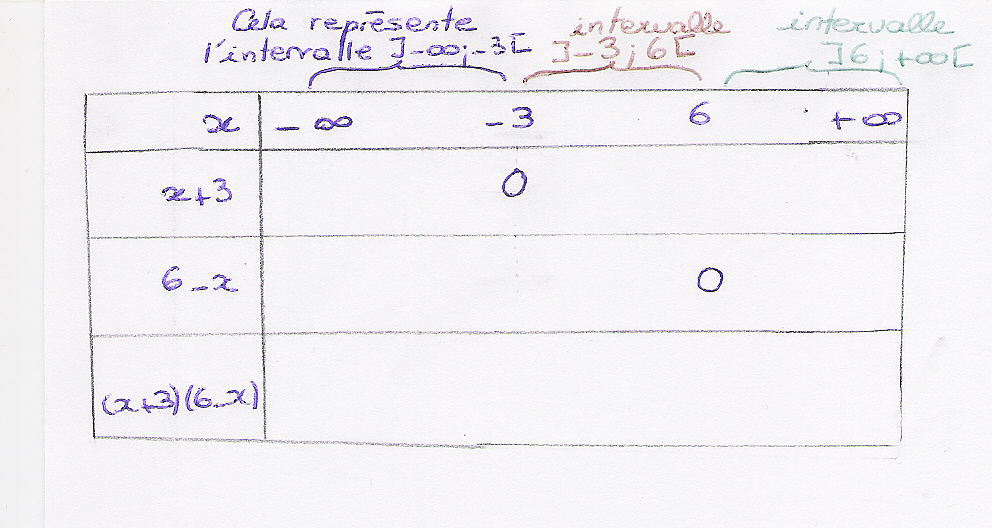
\includegraphics[width=11cm]{images/tab1.jpg}
  \end {center}


  
 \item On r�sout: $x+3>0$
 
 
 $x>\ldots$.
 
      
   Quand $x>-3$, $x+3 \ldots 0$.
   
   Quand $x>-3$, $x+3$ est \ldots \ldots \ldots
  
On note ces informations dans le tableau (sur la ligne $x+3$):

\begin{center}
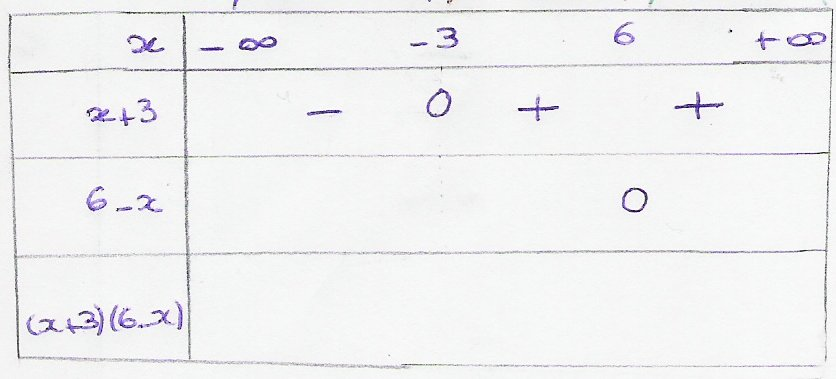
\includegraphics[width=9cm]{images/tab2.jpg}
\end{center}


 \item  On r�sout: $6-x>0$
 
 
 $x\ldots \ldots$.
 
      
   Quand $x<6$, $6-x\ldots 0$.
   
   Quand $x<6$, $6-x$ est \ldots \ldots \ldots 
   
 On note ces informations dans le tableau (sur la ligne $6-x$):

\begin{center}
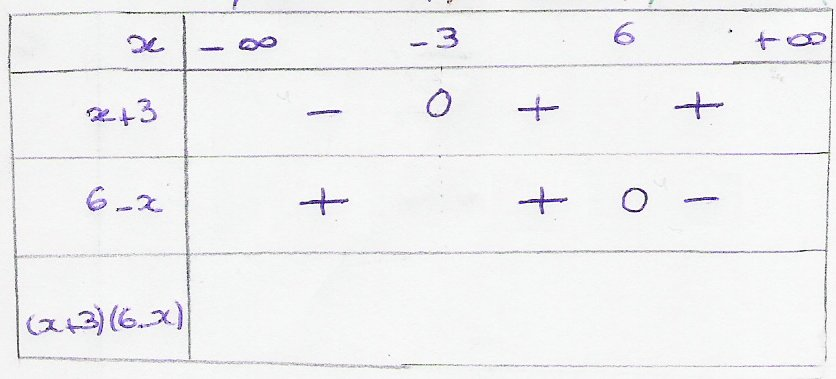
\includegraphics[width=9cm]{images/tab3.jpg}
\end{center}                      
  
 \item Enfin, on compl�te la derni�re ligne en utilisant la r�gle des signes:
 
 \begin{center}
 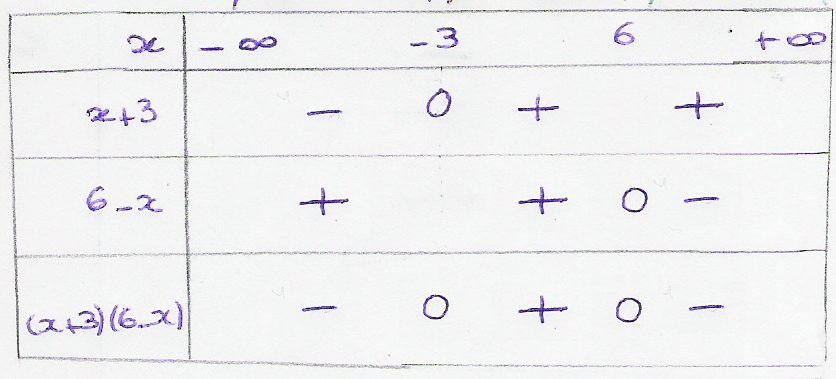
\includegraphics[width=9cm]{images/tab4.jpg}
 
 
 \end{center}
 \item On r�pond � la question: 
 
  Entourer dans votre tableau l'endroit qui indique que $(x-3)(6-x)$ est
  positif ou nul. Cela correspond � quel(s) intervalle(s)?
  
  Compl�ter: $(x-3)(6-x) \geqslant 0$ pour $x \in \ldots \ldots \ldots \ldots$
  
  Donc $\mathcal{D}_{h}=$ \ldots \ldots \ldots \ldots
\end{enumerate} 
  
\end{enumerate}
\subsection*{Applications}

D�terminer l'ensemble de d�finition des fonctions suivantes:


$f(x)=\dfrac{3}{2x-8}$ 

\enskip

 $g(x)=\sqrt{5-7x}$ 

\enskip

$h(x)=x^{2}-7x+19$ 

\enskip

$i(x)= \sqrt{\dfrac{5}{4-x}}$

\enskip

$j(x)= \sqrt{(2x-8)(x+9)}$

\end{document}
